% lonlat.tex

\subsection{Système de coordonnées}

Un point $M$ de la sphère $ S_R = \{ (x,y,z) \in \mathbb{R}^3 \text{ s.t. } x^2 + y^2 + z^2 = R^2\}$ peut être repéré par ses coordonnées longitude-latitude $(\lambda, \theta ) \in ]0, 2\pi ] \times ]- \pi/2, \pi/2 [$. $\lambda$ est la longitude du point donnée par l'angle équatorial et $\lambda$ est l'angle latitudinal (Voir figure \ref{fig:lonlat_sphere}).

\begin{figure}
\begin{center}
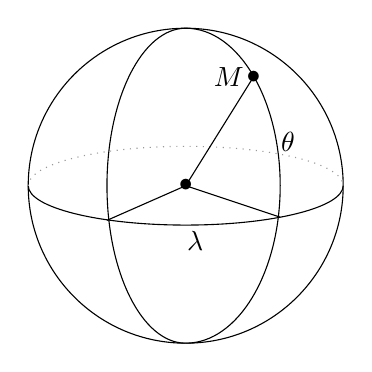
\begin{tikzpicture}[scale=2]
\draw (0,0) circle (1) ;

\draw (-1,0) arc (180:360:1cm and 0.25cm);
\draw (-1,0)[dotted, color=black!40] arc (180:360:1cm and -0.25cm);

\draw (0,1) arc (90:270:0.5cm and 1cm);
\draw (0,1) arc (90:-90:0.6cm and 1cm);

\draw (0,0) node {$\bullet$} ;

\draw (0,0) -- (-0.5,-0.22) ;
\draw (0,0) -- (0.6,-0.2) ;
\draw (0,0) -- (0.43,0.69) ;
\draw (0.43,0.69) node {$\bullet$} ;
\draw (0.43,0.69) node[left]{$M$} ;

\draw (0.06,-0.23) node[below]{$\lambda$} ;
\draw (0.65,0.4) node[below]{$\theta$} ;
\end{tikzpicture}
\end{center}
\caption{Longitude-Latitude}
\label{fig:lonlat_sphere}
\end{figure}


Ainsi $(x,y,z)$ vérifient la relation suivante :

\begin{equation}
\left\lbrace 
\begin{array}{rcl}
x & = & R \cos \theta \cos \lambda \\
y & = & R \cos \theta \sin \lambda \\
z & = & R \sin \theta
\end{array}
\right.
\end{equation}

dès lors on peut construire une base associée sur la sphère : la base covariante $( \mathbf{g}_{\lambda}, \mathbf{g}_{\theta})$ est donnée en $M = (x,y,z) \in S$ par :

\begin{equation}
\mathbf{g}_{\lambda} = \dfrac{\partial M}{\partial \lambda} = \begin{pmatrix}
- R \cos \theta \sin \lambda \\ 
R \cos \theta \cos \lambda \\ 
0
\end{pmatrix} 
\end{equation}

ainsi que 

\begin{equation}
\mathbf{g}_{\theta} = \dfrac{\partial M}{\partial \theta} = \begin{pmatrix}
- R \sin \theta \cos \lambda \\ 
- R \sin \theta \sin \lambda \ \\ 
R \cos \theta
\end{pmatrix} 
\end{equation}

\begin{remarque}
\label{base_lonlat}
On peut normaliser cette base en $\mathbf{e}_{\lambda} = \dfrac{1}{\| \mathbf{g}_{\lambda} \|} \mathbf{g}_{\lambda}$ et $\mathbf{e}_{\theta} = \dfrac{1}{\| \mathbf{g}_{\theta} \|} \mathbf{g}_{\theta}$. Si $\mathbf{F} \in \mathbb{T}S_R$ alors il existe $F_{\lambda}$ et $F_{\theta}$ tels que $\mathbf{F} = F_{\lambda} \mathbf{e}_{\lambda} + F_{\theta} \mathbf{e}_{\theta}$.
\end{remarque}

Ainsi $\mathbf{G}$ le tenseur métrique est :

\begin{equation}
\mathbf{G} = 
\begin{pmatrix}
\mathbf{g}_{\lambda} \cdot \mathbf{g}_{\lambda} & \mathbf{g}_{\lambda} \cdot \mathbf{g}_{\theta} \\
\mathbf{g}_{\theta} \cdot \mathbf{g}_{\lambda} & \mathbf{g}_{\theta} \cdot \mathbf{g}_{\theta}
\end{pmatrix}
 =
\begin{pmatrix}
R^2 \cos \theta & 0 \\
0 & R^2
\end{pmatrix}
\end{equation}

On pose alors $\overline{\mathbf{G}} = det (\mathbf{G}) = R^4 \cos^2 \theta$. La base contravariante $( \mathbf{g}^{\lambda}, \mathbf{g}^{\theta} ) $ est telle que :

\begin{equation}
\left\lbrace 
\begin{array}{rcl}
\mathbf{g}^{\lambda} & = & \mathbf{G}^{1,1} \mathbf{g}_{\lambda} + \mathbf{G}^{1,2} \mathbf{g}_{\theta} \\
\mathbf{g}^{\theta} & = & \mathbf{G}^{2,1} \mathbf{g}_{\lambda} + \mathbf{G}^{2,2} \mathbf{g}_{\theta} \\
\end{array}
\right.
\end{equation}

avec $\mathbf{G}^{i,j} = \left( \mathbf{G}^{-1} \right)_{i,j}$.
De là, il découle :

\begin{equation}
\begin{array}{rcl}
\mathbf{g}^{\lambda} & = & \dfrac{1}{R \cos \theta}  \mathbf{e}_{\lambda} \\
\mathbf{g}^{\theta} & = & \dfrac{1}{R} \mathbf{e}_{\theta}
\end{array}
\end{equation}

Depuis ces vecteurs élémentaires, on peut obtenir des formules pour calculer le gradient, la divergence et le laplacien sphérique ainsi que l'intégrale sur la surface d'une sphère.

\subsection{Opérateurs classiques sur la sphère}

Soit $u$ une fonction de $S_R$ dans $\mathbb{R}$ dérivable pour $\lambda$ et $\theta$. On peut calculer le gradient de $u$ par :

\begin{equation}
\nabla u = \dfrac{\partial u}{\partial \lambda} \mathbf{g}^{\lambda} + \dfrac{\partial u}{\partial \theta} \mathbf{g}^{\theta}
\end{equation}

ce qui se traduit en :

\begin{equation}\label{gradient_lonlat}
\nabla u = \dfrac{1}{R \cos \theta}\dfrac{\partial u}{\partial \lambda} \mathbf{e}_{\lambda} + \dfrac{1}{R} \dfrac{\partial u}{\partial \theta} \mathbf{e}_{\theta}.
\end{equation}

Soit un champ de vecteurs sur la sphère $\mathbf{F} = F_{\lambda} \mathbf{e}_{\lambda} + F_{\theta} \mathbf{e}_{\theta}$ dérivable pour chacune de ses variables sur chacune de ses composantes. Alors 

$$
\left\lbrace 
\begin{array}{rcl}
\mathbf{F} \cdot \mathbf{g^{\lambda}} & = & \dfrac{1}{R \cos \theta} F_{\lambda} \\
\mathbf{F} \cdot \mathbf{g^{\theta}} & = & \dfrac{1}{R} F_{\theta}
\end{array}
\right.
$$

d'où la divergence de $\mathbf{F}$ :

\begin{equation}
\nabla \cdot \mathbf{F} = \dfrac{1}{\sqrt{\overline{\mathbf{G}}}} \left( \dfrac{\partial}{\partial \lambda} \left( \sqrt{\overline{\mathbf{G}}} \mathbf{F} \cdot \mathbf{g}^{\lambda}  \right) +  \dfrac{\partial}{\partial \theta} \left( \sqrt{\overline{\mathbf{G}}} \mathbf{F} \cdot \mathbf{g}^{\theta}  \right)  \right)
\end{equation}

d'où :

\begin{equation}\label{divergence_lonlat}
\nabla \cdot \mathbf{F} = \dfrac{1}{R \cos \theta} \dfrac{\partial}{\partial \lambda}  F_{\lambda} + \dfrac{1}{R \cos \theta} \dfrac{\partial}{\partial \theta} \left( \cos \theta F_{\theta} \right)
\end{equation}

Le laplacien est une composition des deux opérateurs précédents : $\Delta u = \nabla \cdot \nabla u$ :

\begin{equation}\label{laplacien_lonlat}
\Delta u = \dfrac{1}{R^2 \cos^2 \theta} \dfrac{\partial^2 u }{\partial \lambda^2} + \dfrac{1}{R^2 \cos \theta} \dfrac{\partial}{\partial \theta} \left( \cos \theta \dfrac{\partial u}{\partial \theta} \right)
\end{equation}

En plus des opérateurs différentiels courants, on peut donner une formule d'intégration :

\begin{equation}\label{integrale_lonlat}
\gint_{S_R} u = \gint_{\lambda=0}^{2 \pi} \gint_{\theta = - \pi/2}^{\pi/2} u(\lambda, \theta) \underbrace{R^2 \cos \theta}_{\sqrt{\overline{\mathbf{G}}}} d \theta d \lambda
\end{equation}
